\documentclass{article}
\usepackage{graphicx}
\usepackage{amsmath}
\usepackage{amsfonts} 
% or 
\usepackage{amssymb}

\usepackage{tikz}
\usepackage{pgfplots}
\usepgfplotslibrary{fillbetween}
\usetikzlibrary{patterns}

\pgfplotsset{compat = newest}
\usepackage{cancel}
\usepackage[margin=1in]{geometry}
\usepackage{siunitx}
\usetikzlibrary{snakes}
\usepackage{pgflibrarysnakes}
\usetikzlibrary{decorations}

\usetikzlibrary{arrows,automata,positioning}

\usepackage{listings}
\usepackage{color}

\lstset{language=c}

\begin{document}

\section{Signed and Unsigned}

There are three main ways of representing signed integers in binary

\begin{itemize}
	\item{
		\textbf{Sign and Magnitude} --- To represent a negative number in this form we simply take
		the positive number and change the most significant bit to a $1$. For eample $2_{10}$ is $0010_2$ so
		$-2_{10}$ is $1010_2$.
	}
	\item{
		\textbf{1's Compliment} --- To represent a negative number in this form we simply take the positive number
		and invert all of the bits. For example $2_{10}$ is $0010_2$ so $-2_{10}$ is $1101_2$.
	}
	\item{
		\textbf{2's Compliment} --- To represent a negative number in this form we simply take the 1's compliment form and add $1$.
		For example $2_{10}$ is $0010_2$, so the 1's compliment form of $-2_{10}$ (invert all the bits) is $1101_2$. This means
		the 2's compliment form is $1110_2$ ($1101_2 + 0001_2$).
	}
\end{itemize}

\begin{center}
  \begin{tabular}{ | c | c | c | c | }
    \hline
    Decimal & Sign + Mag & 1's Compliment & 2's compliment \\ \hline
    $-2_{10}$ & $1010_2$ & $1101_2$ & $1110_2$\\ \hline
    $-1_{10}$ & $1001_2$ & $1110_2$ & $1111_2$\\ \hline
    $-0_{10}$ & $1000_2$ & $1111_2$ & N/A\\ \hline
    $0_{10}$ & $0000_2$ & $0000_2$ & $0000_2$\\ \hline
    $1_{10}$ & $0001_2$ & $0001_2$ & $0001_2$\\ \hline
    $2_{10}$ & $0010_2$ & $0010_2$ & $0010_2$ \\
    \hline
  \end{tabular}
\end{center}

\subsection{Sign and Magnitude Properties}
The sign and magnitude notation is by far the simplest of the notations.
It retains the property of the least significant bit telling us it's
parity, and it has the property of the largest significant bit telling us
the sign. It is the easiest for us humans to convert to. However this has the side
affect of allowing two ways of encoding $0$ ($+0$, $-0$) and adding them is non trivial.

\begin{center}
  \begin{tabular}{ | c | c | c | c | c | }
    \hline
    Decimal & $\pm$ & $4_{10}$ & $2_{10}$ & $1_{10}$\\ \hline
    $-2_{10}$ & $1$ & $0$ & $1$ & $0$\\ \hline
    $-1_{10}$ & $1$ & $0$ & $0$ & $1$\\ \hline
    $-0_{10}$ & $1$ & $0$ & $0$ & $0$\\ \hline
    $0_{10}$ & $0$ & $0$ & $0$ & $0$ \\ \hline
    $1_{10}$ & $0$ & $0$ & $0$ & $1$\\ \hline
    $2_{10}$ & $0$ & $0$ & $1$ & $0$ \\
    \hline
  \end{tabular}
\end{center}

\subsection{1's Compliment Properties}
Like the sign and magnitude notation, 1's compliment retains the property of
the most significant bit being the sign however it doesn't retain the property of 
the least significant bit denoting the parity. There are still two notations of 
$0$ with 1's compliment though it is much simpler for us to add up.

\begin{center}
  \begin{tabular}{ | c | c | c | c | c | }
    \hline
    Decimal & $-7_{10}$ & $4_{10}$ & $2_{10}$ & $1_{10}$\\ \hline
    $-2_{10}$ & $1$ & $1$ & $0$ & $1$\\ \hline
    $-1_{10}$ & $1$ & $1$ & $1$ & $0$\\ \hline
    $-0_{10}$ & $1$ &  $1$ & $1$ & $1$\\ \hline
    $0_{10}$ & $0$ &  $0$ & $0$ & $0$\\ \hline
    $1_{10}$ & $0$ & $0$ & $0$ & $1$\\ \hline
    $2_{10}$ & $0$ & $0$ & $1$ & $0$ \\
    \hline
  \end{tabular}
\end{center}

\break

\subsubsection{Adding}
When adding a 1's compliment binary number we start by adding normally. Then, at the end,
we add the carry bit from the $-7_{10}$ column to the beggining.

\begin{center}
  \begin{tabular}{c | c | c | c | c }
    Decimal & $-7_{10}$ & $4_{10}$ & $2_{10}$ & $1_{10}$\\ \hline
    $3_{10}$ & $0$ & $0$ & $1$ & $1$\\
    $-1_{10}$ & $1$ & $1$ & $1$ & $0$\\ \hline
    & $0$ &  $0$ & $0$ & $1$\\
	& $1$ & $1$ &\\ \hline
	Add carry bit & & & &  $1$ \\
	$2_{10}$ & $0$ & $0$ & $1$ & $0$ \\ \hline
	& & & $1$ &\\
  \end{tabular}
\end{center}

\subsection{2's Compliment Properties}
With twos compliment we retain both the properties of the least significant bit telling us the parity
and the most significant bit telling us the sign. There are no longer two notations of $0$ and 
we can use a standard, unsigned adder to get the sum of two 2's compliment binary numbers.

\begin{center}
  \begin{tabular}{ | c | c | c | c | c | }
    \hline
    Decimal & $-8_{10}$ & $4_{10}$ & $2_{10}$ & $1_{10}$\\ \hline
    $-2_{10}$ & $1$ & $1$ & $1$ & $0$\\ \hline
    $-1_{10}$ & $1$ & $1$ & $1$ & $1$\\ \hline
    $0_{10}$ & $0$ &  $0$ & $0$ & $0$\\ \hline
    $1_{10}$ & $0$ & $0$ & $0$ & $1$\\ \hline
    $2_{10}$ & $0$ & $0$ & $1$ & $0$ \\
    \hline
  \end{tabular}
\end{center}

\subsubsection{Adding}
When adding a 2's compliment binary number we just add the number normally as shown bellow:

\begin{center}
  \begin{tabular}{c | c | c | c | c }
    Decimal & $-7_{10}$ & $4_{10}$ & $2_{10}$ & $1_{10}$\\ \hline
    $3_{10}$ & $0$ & $0$ & $1$ & $1$\\
    $-1_{10}$ & $1$ & $1$ & $1$ & $1$\\ \hline
    $2_{10}$& $0$ &  $0$ & $1$ & $0$\\
	& $1$ & $1$ & $1$\\
  \end{tabular}
\end{center}

\section{Multiplication}
When multiplying 2 binary numbers we multiply the first number by hte digits of the second number
individually bit shifting to the left by $1$ every time. We then take the sum of these numbers to
get our answer.

\begin{center}
  \begin{tabular}{c | c | c | c | c | c}
    Decimal & $8_{10}$ & $4_{10}$ & $2_{10}$ & $1_{10}$i & shift\\ \hline
    $3_{10}$ & $0$ & $0$ & $1$ & $1$ & \\
    $5_{10}$ & $0$ & $1$ & $0$ & $1$ &\\ \hline
    $3_{10}$& $0$ &  $0$ & $1$ & $1$ & 0\\
    $0_{10}$& $0$ &  $0$ & $0$ & $0$ & 1\\
    $12_{10}$& $1$ &  $1$ & $0$ & $0$& 2\\
    $0_{10}$& $0$ &  $0$ & $0$ & $0$& 3\\ \hline
    $15_{10}$& $1$ &  $1$ & $1$ & $1$\\
  \end{tabular}
\end{center}

\section{Representing Reals}
In computer science there are two main ways of representing real numbers. Fixed point, where a point is placed in the middle of
a set of bits. And floating point which is equivalent to base $2$ scientific notation. Examples of fixed and floating point
binary numbers are shown below:

\begin{center}
  \begin{tabular}{ | c | c | c | c | c | c | c | c | c |}
    \hline
    Decimal & $-8_{10}$ & $4_{10}$ & $2_{10}$ & $1_{10}$ & $0.5_{10}$ & $0.25_{10}$ & $0.125_{10}$ & $0.0625_{10}$\\ \hline
    $-2.375_{10}$ & $1$ & $1$ & $0$ & $1$ & $0$ & $1$ & $1$ & $0$\\ 
    \hline
  \end{tabular}
\end{center}

\begin{gather}
	-6.5_{10} = 0.8125_{10} \times 2_{10}^{3_{10}} = 01101_2 \times 2_{10}^{011_2} \\
	\therefore \\
	-6.5_{10} = {\overbrace{01101}^{\text{Mantissa}}\overbrace{011}^{\text{Exponent}}}_2
\end{gather}

\subsection{Normmalising Floating Point Numbers}
Reals can have many floating point representations in binary, normalising is the process of turning one
repersentation of a real into another with the largest possible mantissa that can repersent that value.
Below, all of the different possible values for $1_{10}$ in a 5 bit signed mantissa and 3 bit signed exponent
are shown below:

\begin{center}
  \begin{tabular}{ | c | c | c | c | c | c | | c | c | c |}
    \hline
    Decimal & $-1_{10}$ & $0.5_{10}$ & $0.25_{10}$ & $0.125_{10}$ & $0.0625_{10}$ & $-4_{10}$ & $2_{10}$ & $1_{10}$\\ \hline
    $1_{10}$ & $0$ & $0$ & $0$ & $1$ & $0$ & $0$ & $1$ & $1$\\ \hline
    $1_{10}$ & $0$ & $0$ & $1$ & $0$ & $0$ & $0$ & $1$ & $0$\\ \hline
    $1_{10}$ & $0$ & $1$ & $0$ & $0$ & $0$ & $0$ & $0$ & $1$\\ 
    \hline
  \end{tabular}
\end{center}
The normalised value for $1_{10}$ is $01000001_2$ as that is the representation where the mantissa has the largest magnitude.
The normalised value for $-1_{10}$ is $10000000_2$ as that is the representation where the mantissa has the largest magnitude.
The normalised value for $-2.5_{10}$ is $10110010_2$ as that is the reperesentation where the mantissa has the largest magnitude.
\\\\
Negative, normalised floats always start with $10$ whereas positive normalised floats always start with $01$.
\subsection{Advantages of each}
\begin{itemize}
	\item Floating Points can represent both massive (size of the universe) and tiny (size of a photon) numbers
		in a small number of bits. However floating point numbers have the issue of floating point
		rounding errors where basic addition and subtraction of floating points can result in a small error in
		the answer, this means they are not suitible for banking where exact values must be known.
	\item Fixed point numbers have the advantage of being able to use the samee basic integer arithemetic operations
		in a processor, this makes them very easy to handle however they can only represent a small range of numbers
		so, unlike floats, they're not as useful in science but are useful in banking.
\end{itemize}

\section{Structured Programming}




\subsection{Unstructured}
When writing an unstructured program it is common to use \lstinline{break} and \lstinline{goto} to jump around to abitrary
blocks of code as. The bellow listing makes use of the \lstinline{goto} statement to endlessly print "Hello, World!"

\begin{lstlisting}

int main() {
loop:
	printf("Hello, World!\n");
	goto loop;
}


\end{lstlisting}

\subsection{Structured}
In structured programming, the flow of our program can be represented in a strict heiarchey. We shouldn't use \lstinline{break} or
\lstinline{goto} to jump around our program, instead we make use of \lstinline{if} and \lstinline{while} statements to provide
selection and iteration instead of conditionally jumping. We also use subrountines instead of blocks to split up our program.
The previous listing has been rewritten as a structured program.

\begin{lstlisting}
int main() {
	while (true) {
		printf("Hello, World!\n");
	}
}
\end{lstlisting}
Compilers of structured programming languages internally map structured programming patterns to unstructured programming patterns.
This is because CPU architectures tend not to deal with the complexity that having to process structured machine code
would bring. 
\\
Assembly and intermediate languages such as AT\&T assembly and LLVM IR do not support structured programming, they require
loops and conditions to be unrolled into conditional breaks.

\subsection{Advantages}
Structured programming makes code much easier to read and debug, thus reducing time developers spend on a problem.

\subsection{Disadvantages}
Structured programming removes some opportunity for cleaver code, thus structured programs tend to be slower than
unstructured programs. However, modern compilers make this difference negligible thanks to advanced optimisation 
techniques.

\section{Finite State Machines}


\begin{center}
    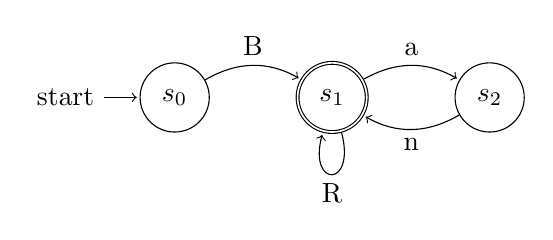
\begin{tikzpicture}[shorten >=1pt,node distance=2cm,on grid,auto]

        \node[state,initial] (s_0) {$s_0$};
        \node[state,accepting] (s_1) [right of=s_0] {$s_1$};
        \node[state] (s_2) [right of=s_1] {$s_2$};

        \path[->]
        (s_0) edge [bend left] node {B}  (s_1)
        (s_1) edge [loop below] node {R}  ()
        (s_1) edge [bend left] node {a}  (s_2)
        (s_2) edge [bend left] node {n}  (s_1);

    \end{tikzpicture}

    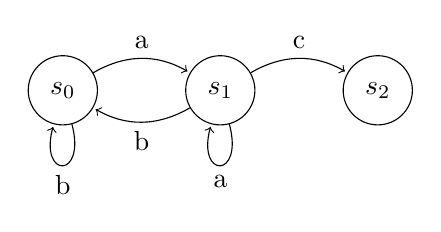
\begin{tikzpicture}[shorten >=1pt,node distance=2cm,on grid,auto]

        \node[state] (s_0) {$s_0$};
        \node[state] (s_1) [right of=s_0] {$s_1$};
        \node[state] (s_2) [right of=s_1] {$s_2$};

        \path[->]
        (s_0) edge [bend left] node {a}  (s_1)
        (s_1) edge [bend left] node {b}  (s_0)
        (s_0) edge [loop below] node {b}  ()
        (s_1) edge [loop below] node {a}  ()
        (s_1) edge [bend left] node {c}  (s_2);

    \end{tikzpicture}

    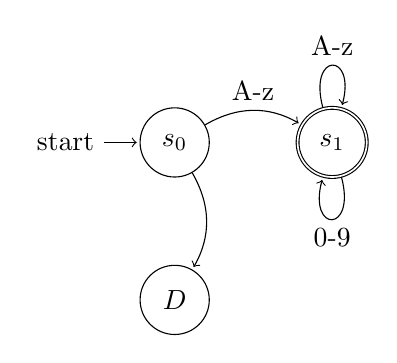
\begin{tikzpicture}[shorten >=1pt,node distance=2cm,on grid,auto]

        \node[state,initial] (s_0) {$s_0$};
        \node[state,accepting] (s_1) [right of=s_0] {$s_1$};
        \node[state] (D) [below of=s_0] {$D$};

        \path[->]
        (s_0) edge [bend left] node {}  (D)
        (s_0) edge [bend left] node {A-z}  (s_1)
        (s_1) edge [loop below] node {0-9}  ()
        (s_1) edge [loop above] node {A-z}  ();

    \end{tikzpicture}
\end{center}

\end{document}
